\chapter{Visualising}
\label{chapter:visualising}

\section{Simple dataframe plots}

One of the simplest ways of visualising data that is in a pandas dataframe is just to call the \code{plot()} method of the dataframe.

To see how this works, we first need to create a dataframe.

\begin{pycode}
    import pandas as pd
    data = {"city":['Brisbane','Sydney','Christchurch','Singapore','Los Angeles'],
            "rating":[4.5,4.2,4.7,4.3,3.9]}
    df = pd.DataFrame(data).set_index('city')
    print(df)
\end{pycode}

\begin{verbatim}
    city          rating
    Brisbane         4.5
    Sydney           4.2
    Christchurch     4.7
    Singapore        4.3
    Los Angeles      3.9
\end{verbatim}


\begin{pycode}
    chart = df.plot(kind='bar')
\end{pycode}

\begin{figure}[!h]
    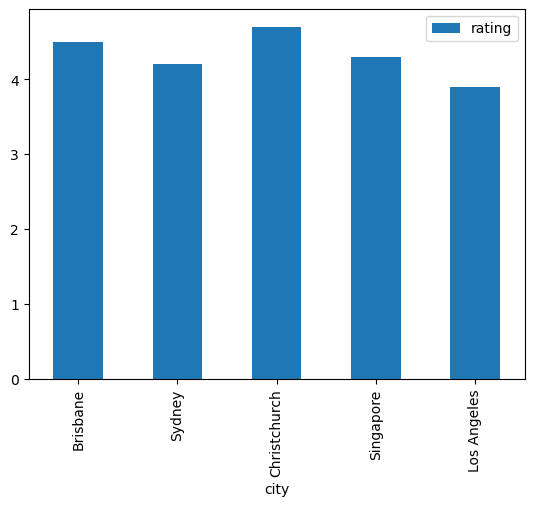
\includegraphics[width=0.5\textwidth]{graphics/simple_bar.png}
\end{figure}